\documentclass{article}
\usepackage[utf8]{inputenc}
\usepackage[margin=1in]{geometry}
\usepackage{amsmath, amsfonts}
\usepackage{fancyhdr}
\usepackage{multicol}
\usepackage{graphicx}
\usepackage[inline]{enumitem}
\graphicspath{ {images/} }
\pagestyle{empty}
\fancyhf{}
\cfoot{\thepage}
\pagenumbering{gobble}

\lhead{MATB42: Assignment \#7}
\rhead{
Poon, Keegan\\
1002423727\\
Mar 13th 2018}
\newcommand{\norm}[1]{\| #1 \|}
\newcommand{\deriv}[1]{\frac{d}{d #1}}
\newcommand{\parti}[1]{\frac{\partial}{\partial #1}}
\renewcommand{\headrulewidth}{0pt}
\newcommand{\gam}{\boldsymbol{\gamma}}
\begin{document}

\thispagestyle{fancy}

\begin{enumerate}
    \item
    \begin{enumerate}
        \item Find an equation of the tangent plane to the surface $S$ defined parametrically by $\boldsymbol \Phi(u, v) = (u^2 + v,\ v,\ u+v^2)$ at the point (9,0,3).
        \begin{align*}
            &v = 0 & &u + v^2 = 3 \implies u = 3&
        \end{align*}
        \begin{align*}
            \boldsymbol \phi_u &= (2(3), 0, 1) \\
            \boldsymbol \phi_v &= (1,1,2(0)) \\
            \boldsymbol \phi_u \times \boldsymbol \phi_v &= (-1,1,6) \\
        \end{align*}
        So the tangent plane can be given by
        \begin{align*}
            0 &= ((x - 9, y, z - 3) \cdot (-1,1,6)) \\
            0 &= (9 - x + y + 6z - 18) \\
            9 &= -x + y + 6z \\
        \end{align*}
        \item Use symbolic algebra software to sketch the surface $S$ and its tangent plane from part (a).
        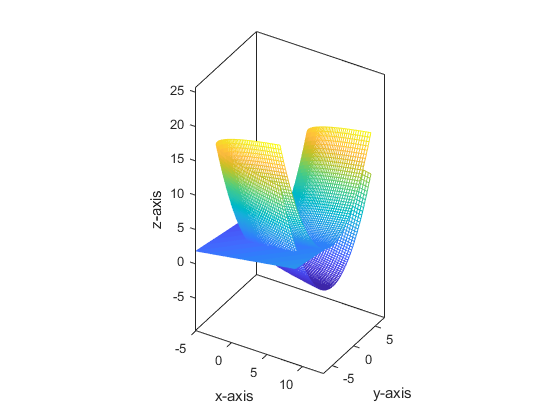
\includegraphics[width=\textwidth]{b42-a7-1b}
    \end{enumerate}

    \item Use a surface integral to find the area of the triangle in $\mathbb{R}^3$ with vertices (1,1,0), (1,2,1) and (3,3,2).

    \item Calculate the surface area of the piece of the cone $x^2+y^2-z^2 =0$ which lies outside the cylinder $x^2 + y^2 = 4$.

    \item
    \begin{enumerate}
        \item Find the area of the portion of the unit sphere that is cut out by the cone $z = \sqrt{x^2+y^2}$.

        (cf. page 391, \#10)

        \item Find the area of the portion of the cone $z = \sqrt{x^2+y^2}$ that is cut out by the unit sphere.
    \end{enumerate}

    \item Let $\boldsymbol \Phi : D \subset \mathbb{R}^2 \rightarrow \mathbb{R}^3$ be a parametrization of a 2-dim surface $S$ in $\mathbb{R}^3$.
    \begin{enumerate}
        \item Set
        \begin{align*}
            & E = \norm{\boldsymbol \phi_u}^2,& &F = \boldsymbol \phi_u \cdot \boldsymbol \phi_v, & & G = \norm{\boldsymbol \phi_v}^2,
        \end{align*} 
        Show that the surface area of $S$ is 
        \[ A(S) = \iint_D \sqrt{EG - F^2}\,dA \]
        
        \begin{align*}
            \iint_D \sqrt{EG - F^2}\,dA &= \iint_D \sqrt{\norm{\boldsymbol \phi_u}^2 \norm{\boldsymbol \phi_v}^2 - (\boldsymbol \phi_u \cdot \boldsymbol \phi_v)^2} \, dA \\
            &= \iint_D \sqrt{(\norm{\boldsymbol \phi_u}\norm{\boldsymbol \phi_v})^2 - (\norm{ \boldsymbol \phi_u} \norm{\boldsymbol \phi_v})^2 \cos^2\theta }\, dA & \text{Where $\theta$ is the angle between $\boldsymbol \phi_u$ and $\boldsymbol \phi_v$.}\\
            &= \iint_D \sqrt{(\norm{\boldsymbol \phi_u}\norm{\boldsymbol \phi_v})^2 (1 - \cos^2\theta) } \, dA \\
            &= \iint_D \sqrt{(\norm{\boldsymbol \phi_u}\norm{\boldsymbol \phi_v})^2 (\sin^2\theta) } \, dA \\
            &= \iint_D \sqrt{\norm{\boldsymbol \phi_u \times \boldsymbol \phi_v)^2} } \, dA \\
        \end{align*} 
        \item What does the formula for $A(S)$ become if the vectors $\boldsymbol \phi_u$ and $\boldsymbol \phi_v$ are orthogonal?
        \item Use parts (a) and (b) to compute the surface area of a sphere of radius $a$.

        (cf. Marsden \& Tromba, page 399, \# 23.)
    \end{enumerate}
    \item For each of the following surfaces $S$, sketch $S$ (using symbolic software) and evaluate the surface integral $\int_S f \, dS$, where $f(x,y,z) = x$.
    \begin{enumerate}
        \item $S$ is that part of the surface $y=4-x^2$ between $z = 0$ and $z = 1$, with $y\geq 0$.
        \item $S$ is the upper half of the unit sphere centered at the origin.
        \item $S$ is that part of the surface $x = \sin y$ with $0 \leq y \leq \pi$ and $0 \leq z \leq 2$.
    \end{enumerate}

    \item Find the mass of the metallic surface $S$ given by $\displaystyle z = 1 - \frac{x^2 + y^2}{2}$ with $0 \leq x \leq 1$, $0 \leq y \leq 1$, if the mass density at $(x,y,z) \in S$ is given by $m(x,y,z) = xy$.
\end{enumerate}
\end{document}
